\subsection{Relaciones de Dependencia}

Las relaciones de dependencia describen la forma en que los elementos apoyan o son utilizados por otros elementos.  Se distinguen tres tipos de relaciones de dependencia:
\begin{itemize}
	\item La relación de servicio representa una dependencia de control, denotada por una línea sólida.
	\item La relación de acceso representa una dependencia de datos, denotada por una línea discontinua.
	\item La relación de influencia es el tipo de dependencia más débil, utilizada para modelar cómo los elementos de motivación son influenciados por otros elementos.
\end{itemize}
Obsérvese que, aunque la notación de estas relaciones se asemeja a la notación de la relación de dependencia en UML, estas relaciones tienen significados distintos en la notación ArchiMate y (normalmente) apuntan en la dirección opuesta.

\begin{table}[h!]
	\subsubsection{Elementos}
	\begin{center}
		\begin{tabular}{| c | l | l |}
			\hline
			Concepto & Descripción & Representación \\ \hline
			
			Sirve 
			&
			\begin{tabular}{m{12em}}
				Modela que un elemento proporciona
				su funcionalidad a otro elemento.
			\end{tabular}
			& 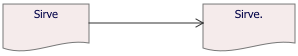
\includegraphics[width=0.4\linewidth]{imgs/relaciones/sirve}
			\\\hline
			
			Influencia
			& 
			\begin{tabular}{m{12em}}
				Modelos en los que un elemento afecta la aplicación o el logro
				de algún elemento de motivación.
			\end{tabular}
			& 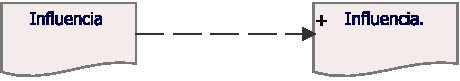
\includegraphics[width=0.4\linewidth]{imgs/relaciones/influencia}
			\\\hline
			
			Acceso
			& 
			\begin{tabular}{m{12em}}
				Modela la capacidad de los elementos
				de comportamiento y estructura activa
				para observar o actuar sobre los
				elementos de estructura pasiva.
			\end{tabular}
			& 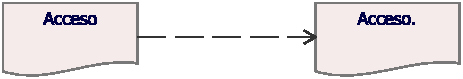
\includegraphics[width=0.4\linewidth]{imgs/relaciones/acceso}
			\\\hline
			
			Acceso Bidireccional
			& 
			\begin{tabular}{m{12em}}
				Modela la capacidad de los elementos
				de comportamiento y estructura activa
				para observar o actuar sobre los
				elementos de estructura pasiva y viceversa.
			\end{tabular}
			& 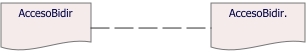
\includegraphics[width=0.4\linewidth]{imgs/relaciones/accesobi}
			\\\hline
			
		\end{tabular}
		\caption{Relaciones de dependencia}
		\label{tab:dependencia}
	\end{center}
\end{table}